\documentclass[a4paper,10pt]{article}
\usepackage[utf8]{inputenc}
\usepackage[english]{babel}
\usepackage{geometry}
\usepackage[T1]{fontenc}
\usepackage{float}
\usepackage{multirow}
\usepackage{booktabs}
\usepackage{chemfig}
\usepackage{amsmath}
\usepackage{xcolor}
\usepackage{pxfonts}
\usepackage{tikz}

\title{Old Xtext Tutorial}
\author{}



\newcommand{\gerquot}[1]{\glqq#1\grqq}
\newcommand{\dashAndSpace}{\textendash \space}
\newcommand{\dashAndSpaceSeq}[1]{\dashAndSpace#1 \textendash}

\newcommand{\DSL}{domain specific language}
\newcommand{\CFG}{context-free grammar}
\newcommand{\IUPAC}{International Union of Pure and Applied Chemistry}
\newcommand{\EMF}{Eclipse Modeling Framework}

\newcommand{\ProjectName}{MyDSLProject}
\newcommand{\ScreenshotWidth}{0.975}

%%%%% %%%%% %%%%% %%%%% %%%%% %%%%% %%%%% %%%%%                %%%%% %%%%% %%%%% %%%%% %%%%% %%%%% %%%%% %%%%%
%%%%% %%%%% %%%%% %%%%% %%%%% %%%%% %%%%% %%%%% BEGIN document %%%%% %%%%% %%%%% %%%%% %%%%% %%%%% %%%%% %%%%%
%%%%% %%%%% %%%%% %%%%% %%%%% %%%%% %%%%% %%%%%                %%%%% %%%%% %%%%% %%%%% %%%%% %%%%% %%%%% %%%%%
\begin{document}

\maketitle

\section{Introduction}\label{s:Introduction}
The \EMF\space can be used to create a meta model for \DSL s. One part of such a model is the Ecore file. A Ecore file holds information about the defined classes and their relationships. Eclipse has a graphical editor to work with them. In this tutorial the main steps \dashAndSpaceSeq{from the project creation up to the data generation} will be explained. We assume, that Eclipse\footnote{For the tutorial Version 2023-09 (4.29.0) was used. Newer versions should also work.} is already installed with the Ecore tools.

\subsection{Creation of a modeling project}\label{ss:CreationModelingProject}
After Eclipse was started, the usage of the proper perspective for modeling projects is recommended. The modeling perspective can be opened via the main drop down menu \emph{Window > Perspective > Open Perspective > Other...} Choose the entry \gerquot{Modeling}. See: figure \ref{fig:SSPerspectiveChange}

\begin{figure}[H]
\centering
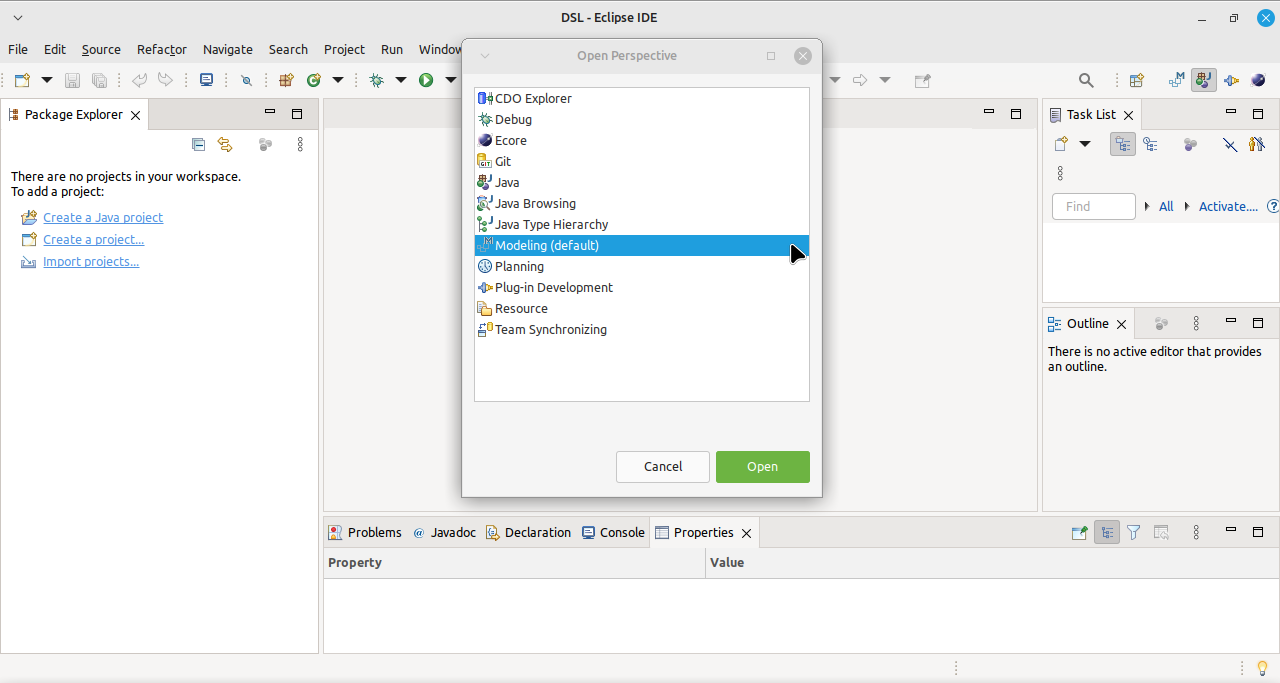
\includegraphics[width=\ScreenshotWidth\textwidth]{./Screenshots/SS_2.png}
\caption{Perspective change to \gerquot{Modeling}.}
\label{fig:SSPerspectiveChange}
\end{figure}

With a right mouse click on the free space in the model explorer a new Modeling project can be created. (Figure \ref{fig:SSNewModellingProject}). We named the project \emph{\ProjectName}.

\begin{figure}
\centering
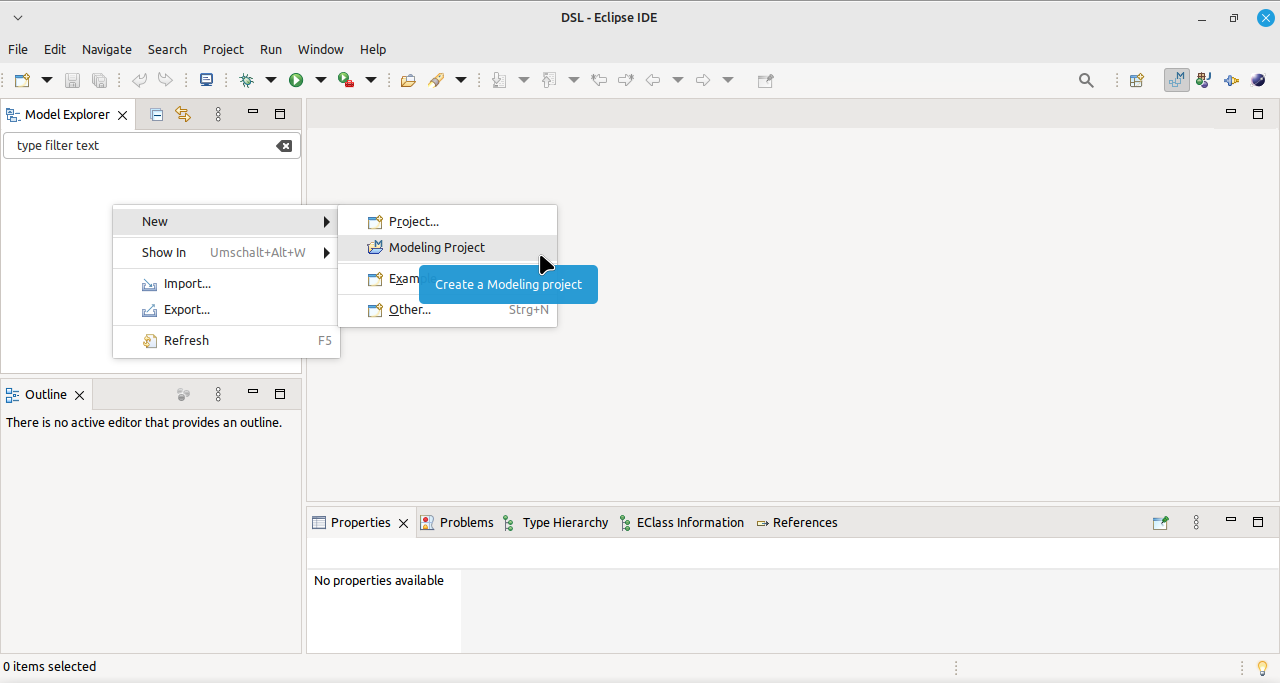
\includegraphics[width=\ScreenshotWidth\textwidth]{./Screenshots/SS_3.png}
\caption{Creation of a new Modeling project.}
\label{fig:SSNewModellingProject}
\end{figure}

For the future work we need an Ecore file. This file can be created with a right click on the project in the model explorer. Via \emph{New > Other...} the wizard for a new file can be opened:

\begin{figure}[H]
\centering
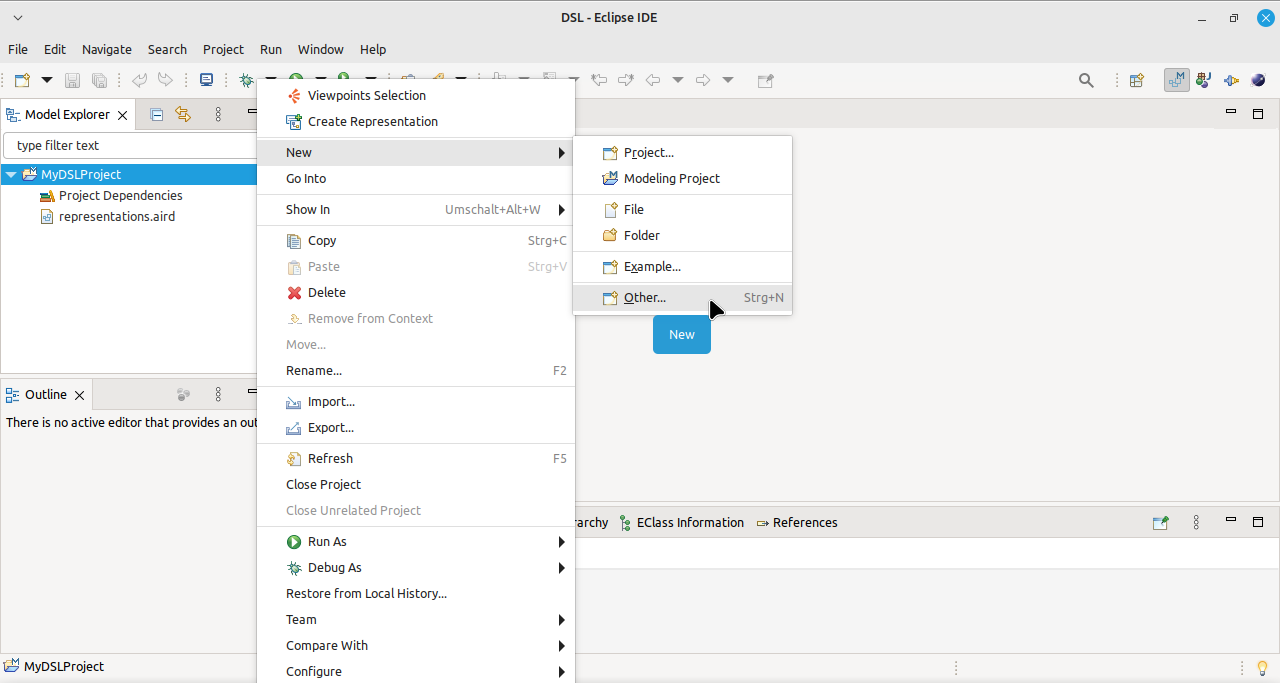
\includegraphics[width=\ScreenshotWidth\textwidth]{./Screenshots/SS_4.png}
\caption{Open the wizard for a new Ecore file.}
\label{fig:SSNewEcoreModel1}
\end{figure}

Inside the wizard is a folder named \gerquot{\EMF}. In this is an entry for a Ecore model. See figure \ref{fig:SSNewEcoreModel2}. We named the Ecore file \emph{My.ecore}

\begin{figure}[H]
\centering
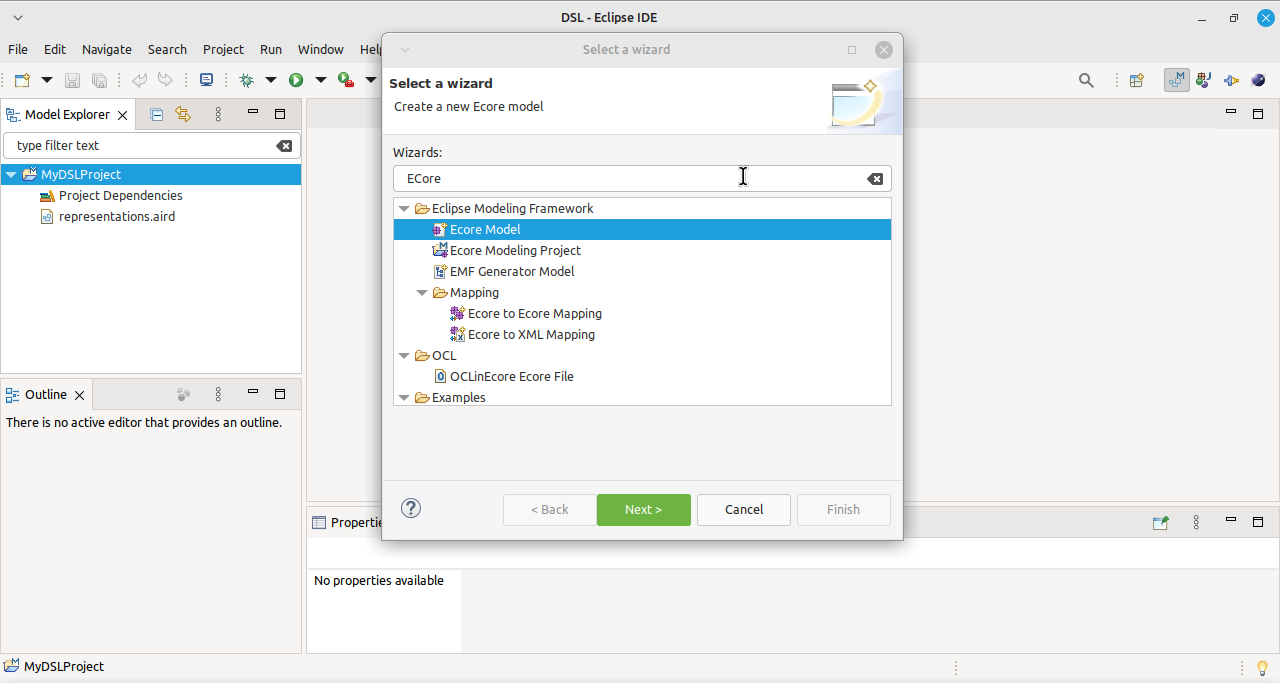
\includegraphics[width=\ScreenshotWidth\textwidth]{./Screenshots/SS_5.png}
\caption{Choosing the Ecore Model in the wizard.}
\label{fig:SSNewEcoreModel2}
\end{figure}

By default the textual Ecore editor will be opened. To use the graphical editor, we need to initialize the Ecore diagram first. This can be done with a right click on the Ecore file. There is a menu entry with the name \gerquot{Initialize Ecore Diagram...}. See: figure \ref{fig:SSInitEcoreDiagram}

\begin{figure}[H]
\centering
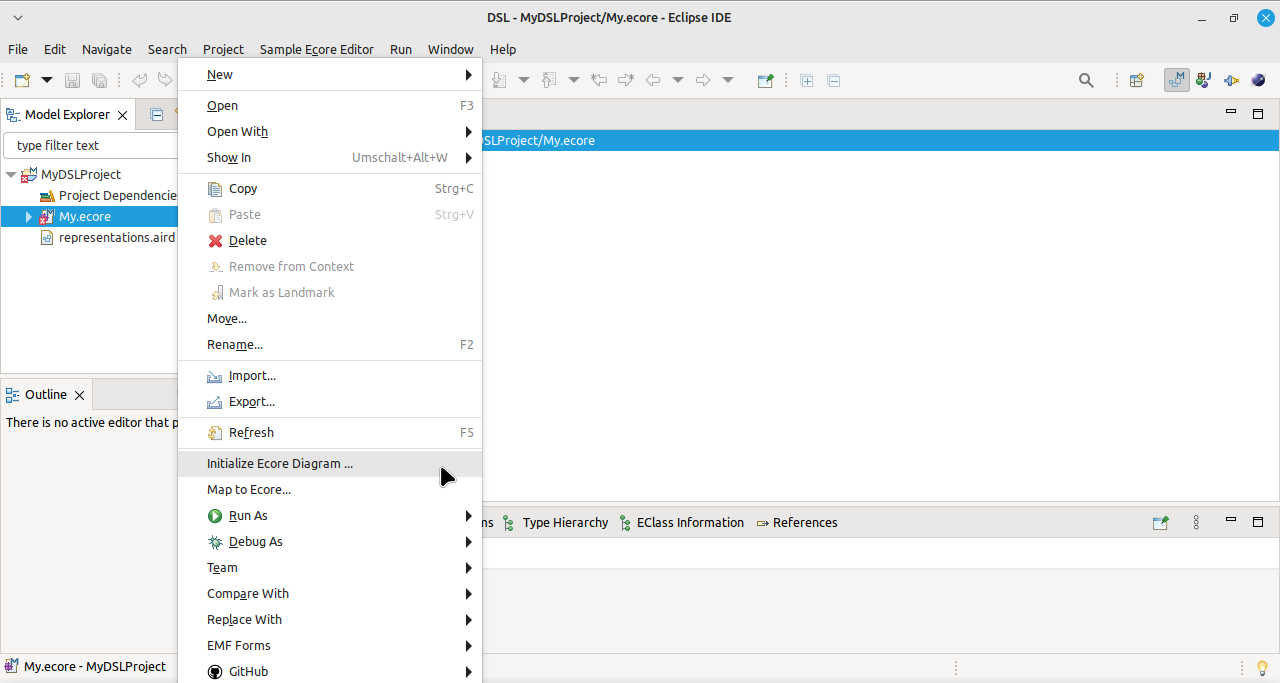
\includegraphics[width=\ScreenshotWidth\textwidth]{./Screenshots/SS_7.png}
\caption{Initialize the Ecore Diagram to use the graphical editor for this file.}
\label{fig:SSInitEcoreDiagram}
\end{figure}

Now a representation of the Ecore file can be selected. In our case the first entry \gerquot{Entities in a Class Diagram} is used. $ \rightarrow $ figure \ref{fig:SSWizardEcoreRepresentations}

\begin{figure}[H]
\centering
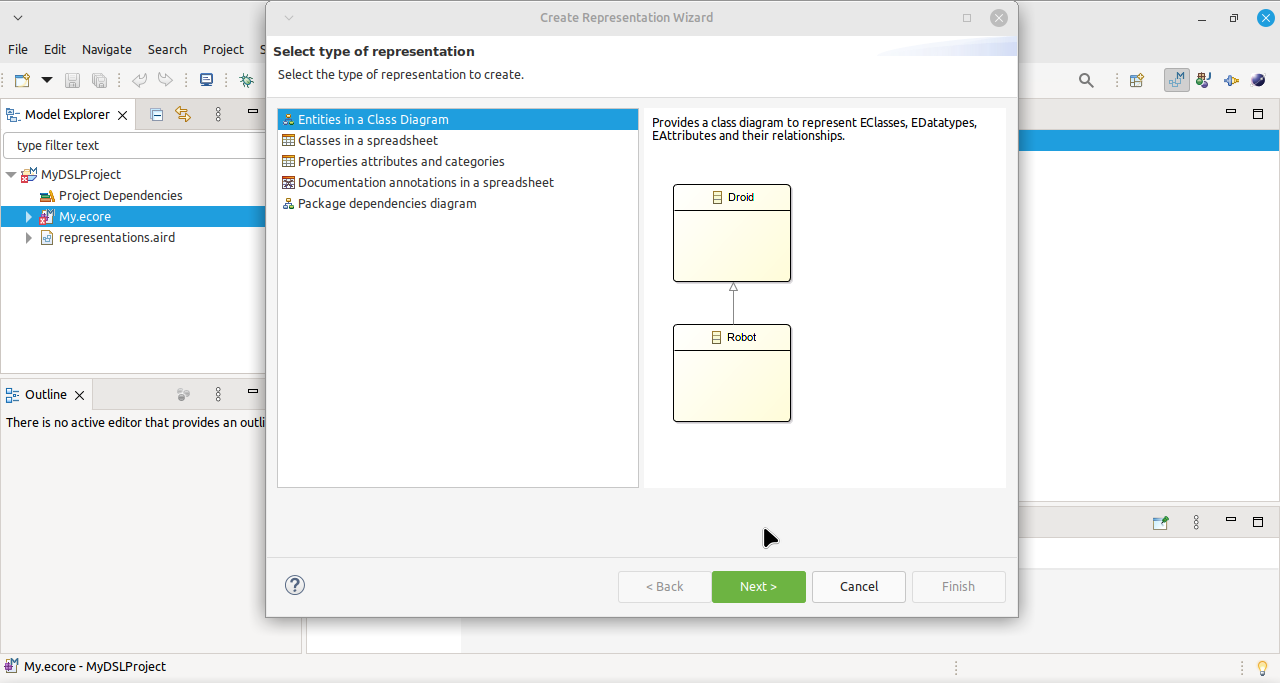
\includegraphics[width=\ScreenshotWidth\textwidth]{./Screenshots/SS_8.png}
\caption{Opened wizard with different representations of an Ecore file.}
\label{fig:SSWizardEcoreRepresentations}
\end{figure}

After selecting this entry, the graphical editor will be opened. By now there are no entities. On the right side is a menu called \gerquot{Palette}. Here under \emph{Classifier > Class} new classes can be created. On figure \ref{fig:SSGraphicalEcoreEditorWithTwoNewClasses} two classes with the name \gerquot{NewEClass1} and \gerquot{NewEClass2} were created.

\begin{figure}[H]
\centering
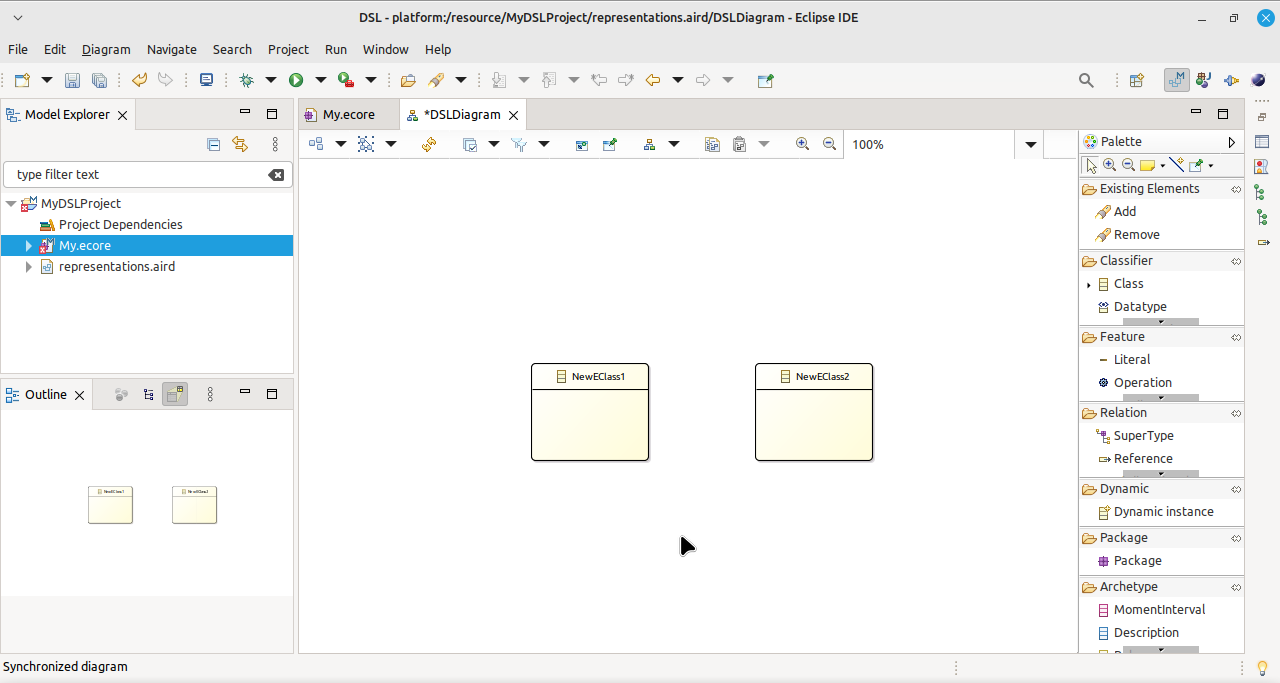
\includegraphics[width=\ScreenshotWidth\textwidth]{./Screenshots/SS_10.png}
\caption{graphical Ecore editor with two new classes.}
\label{fig:SSGraphicalEcoreEditorWithTwoNewClasses}
\end{figure}

With an double left click all properties of a selected class can be shown and altered. We renamed the classes in \gerquot{MyClass1} and in \gerquot{MyClass2}. Under \emph{Classifier > Enumeration} an new enumeration is creatable. (Figure \ref{fig:SSShowNewEnumerationMenuEntry}). We named the new enumeration \gerquot{MyEnum1}.

\begin{figure}[H]
\centering
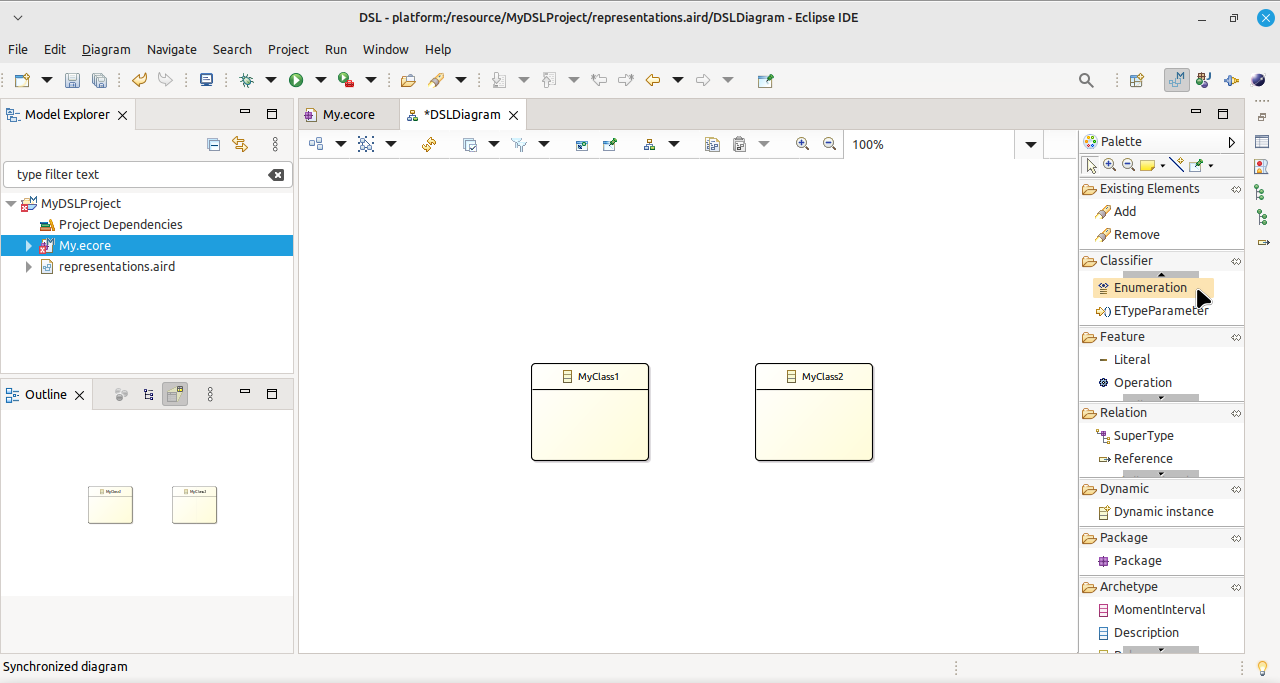
\includegraphics[width=\ScreenshotWidth\textwidth]{./Screenshots/SS_12.png}
\caption{Under Classifier is also for example an entry for new enumerations.}
\label{fig:SSShowNewEnumerationMenuEntry}
\end{figure}

After creating the enumeration, there is no value in it \dashAndSpace not even a default value. To insert new entries a menu like in figure \ref{fig:SSEnumMenuForNewEntries} will appear, when the mouse is in the enumeration.

\begin{figure}[H]
\centering
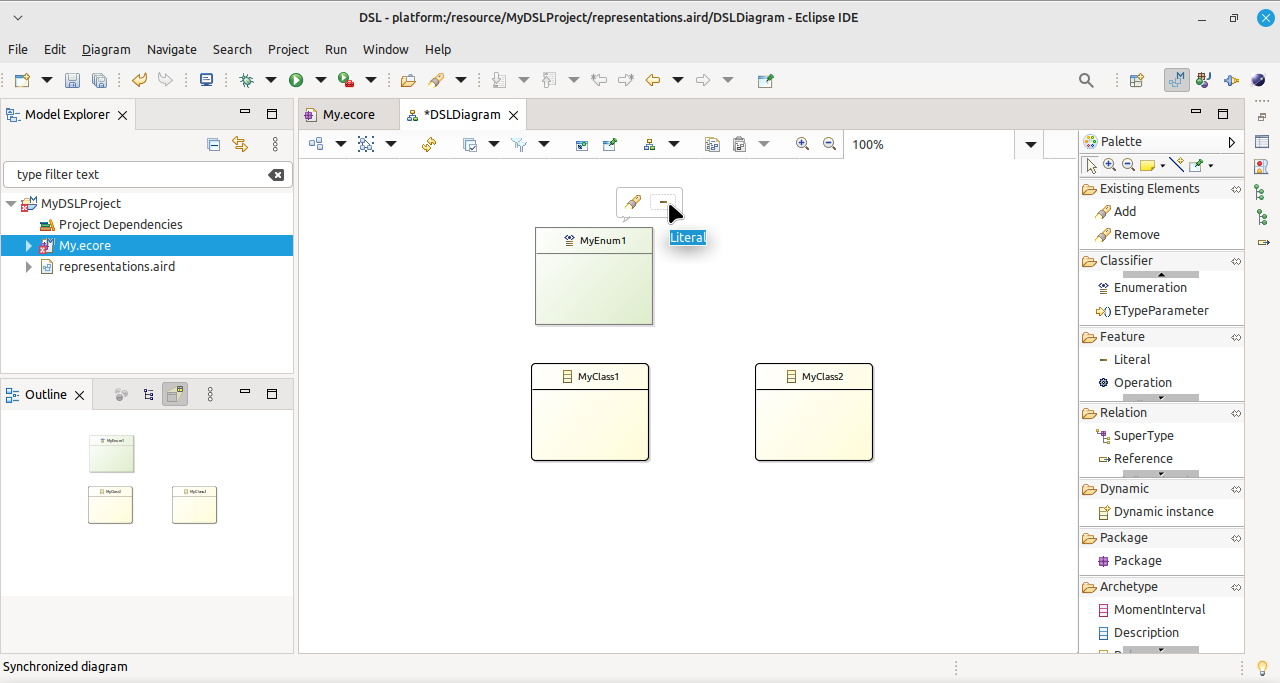
\includegraphics[width=\ScreenshotWidth\textwidth]{./Screenshots/SS_13.png}
\caption{Enumeration with opened menu to insert new entries.}
\label{fig:SSEnumMenuForNewEntries}
\end{figure}

In the same way new attributes can be added to a class. (See: figure \ref{fig:SSClassMenuForNewEntries})

\begin{figure}[H]
\centering
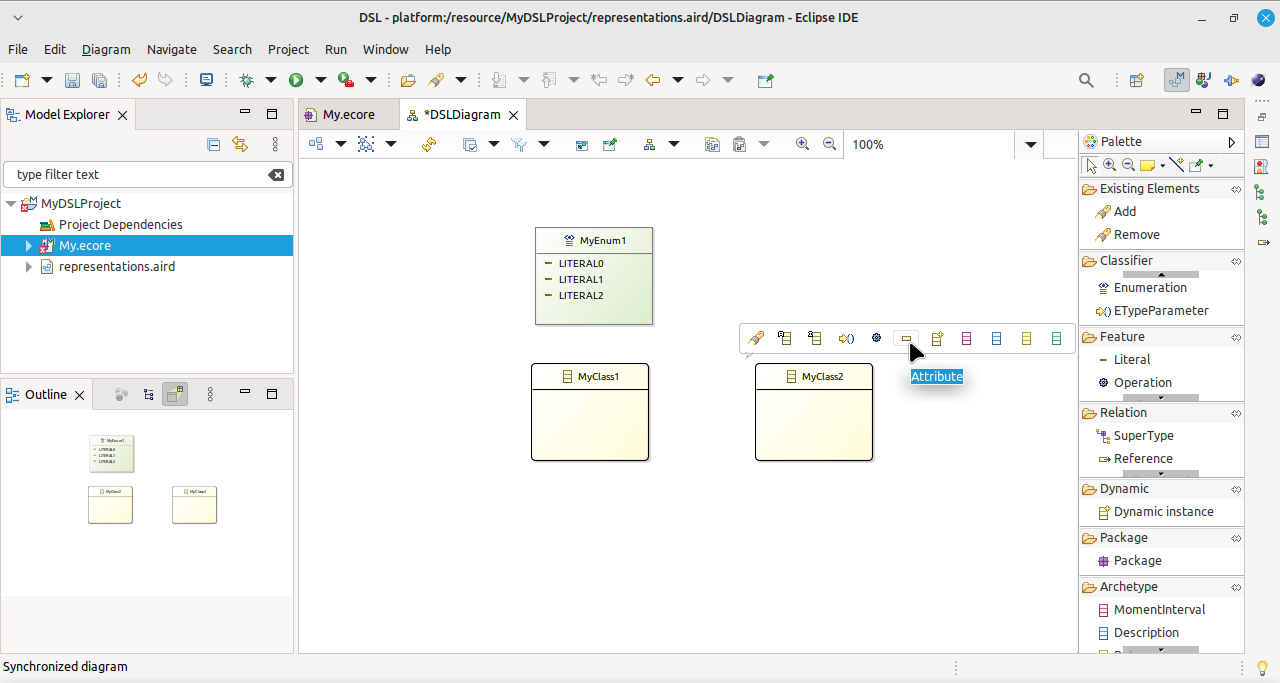
\includegraphics[width=\ScreenshotWidth\textwidth]{./Screenshots/SS_14.png}
\caption{Class with opened menu to insert new attributes.}
\label{fig:SSClassMenuForNewEntries}
\end{figure}

Instead of inserting directly a new object like with enumerations, a window with the new properties of the new attribute will appear. To use an self-defined object, the button with the three dots can be used. $\rightarrow$ Figure: \ref{fig:SSNewAttribute}

\begin{figure}[H]
\centering
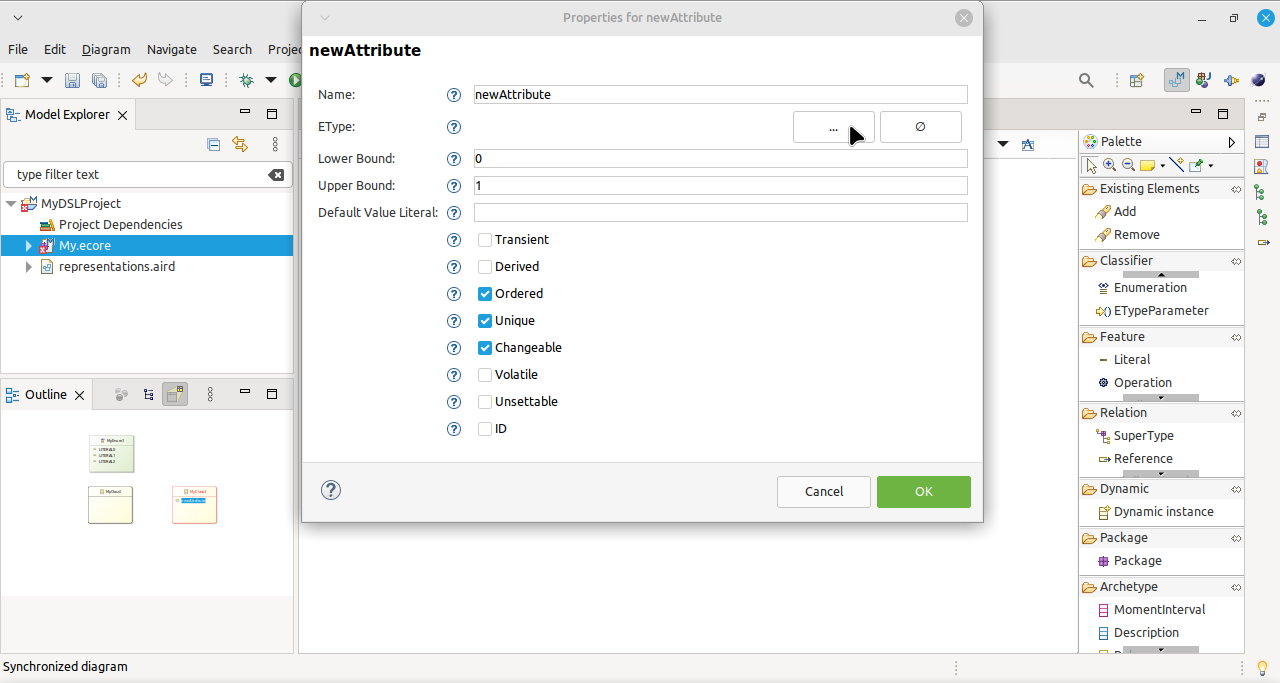
\includegraphics[width=\ScreenshotWidth\textwidth]{./Screenshots/SS_15.png}
\caption{Properties window for the new attribute.}
\label{fig:SSNewAttribute}
\end{figure}

In the list all possible types will be listed. Almost all of them are defined by the \EMF. To find our enumeration, the search function should be used. (Figure: \ref{fig:SSSelectionWindowOfAnAttributesType})

\begin{figure}[H]
\centering
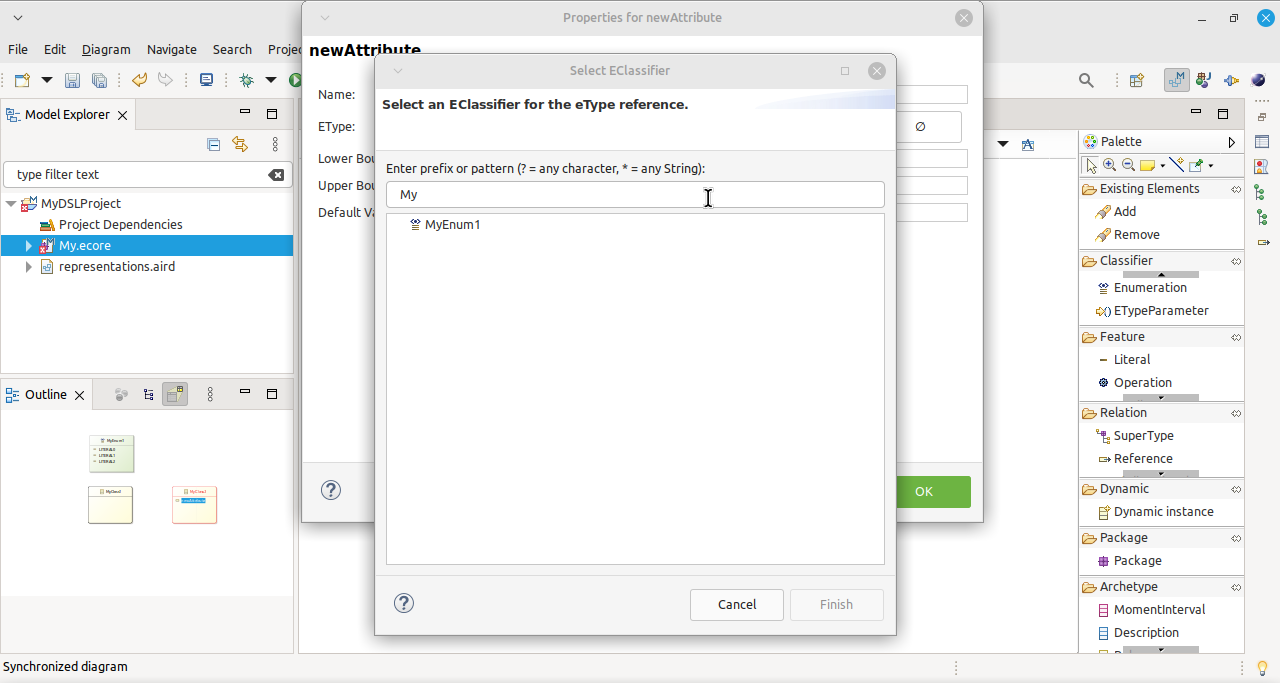
\includegraphics[width=\ScreenshotWidth\textwidth]{./Screenshots/SS_16.png}
\caption{Properties window for the new attribute.}
\label{fig:SSSelectionWindowOfAnAttributesType}
\end{figure}

After clicking on \gerquot{OK}, the new attribute will be created. The new attribute will get a default value, if in the selected type a default value was set. In an enumeration the first entry will be select as default value.\footnote{This behaviour can be changed. In normal cases it is a good practice for readability to set the default value always on the first position.} So the new attribute \gerquot{newAttribute} was get the default value \gerquot{LITERAL0}.

\noindent Usually classes have relationships to each other. If we for example need an composition between to classes this can be added via the menu entry \emph{Relation > Composition}. After selecting this entry two classes needs to be selected.

\begin{figure}[H]
\centering
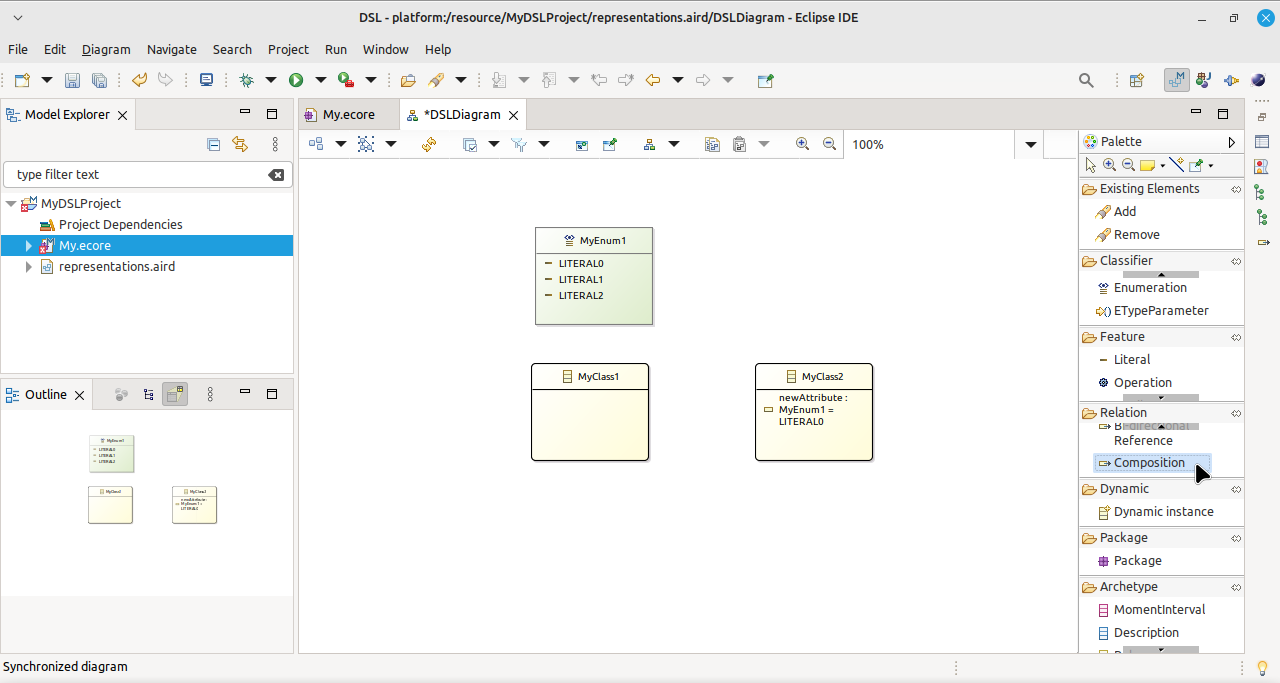
\includegraphics[width=\ScreenshotWidth\textwidth]{./Screenshots/SS_17.png}
\caption{Menu entry to add a composition relation for classes.}
\label{fig:SSMenuForSelectionOfAComposition}
\end{figure}

For a composition a cardinality \emph{0..*} from the first selected to the second class will be added by default. After selecting the relation with the properties menu on the right side (see figure \ref{fig:SSPropertiesButtonOnRightSide}) the cardinality can be changed.

\begin{figure}[H]
\centering
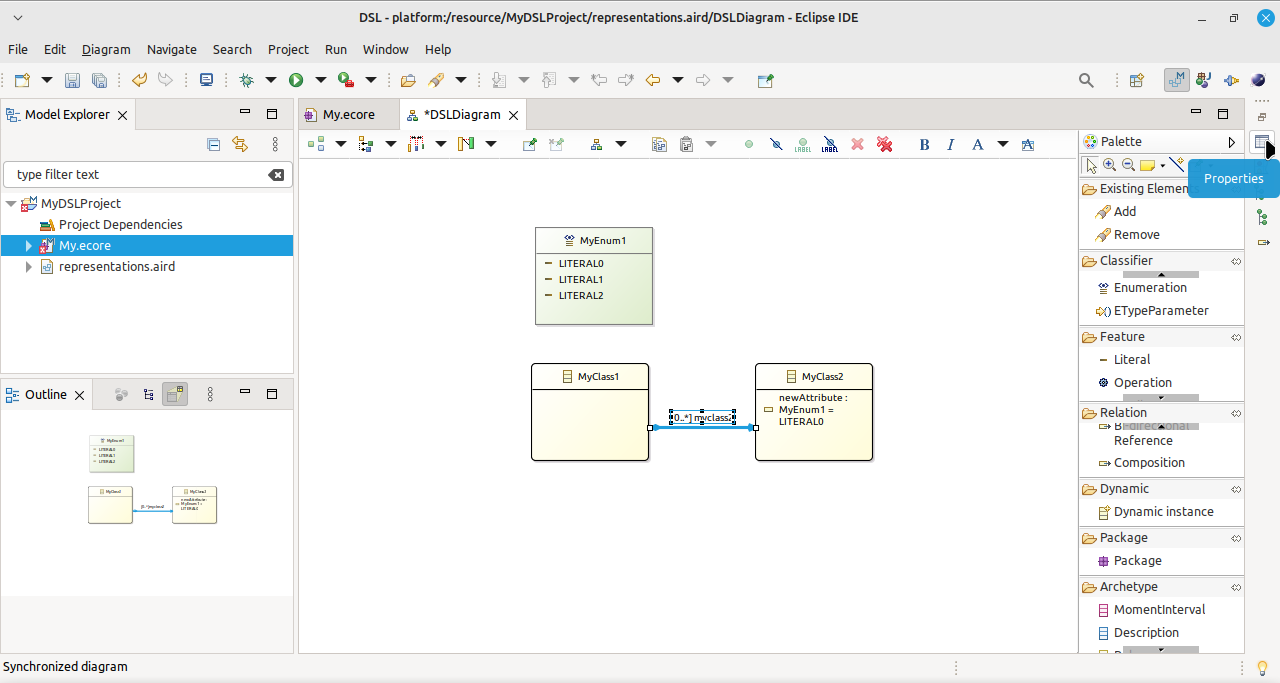
\includegraphics[width=\ScreenshotWidth\textwidth]{./Screenshots/SS_19.png}
\caption{The properties menu is a small button on the right side.}
\label{fig:SSPropertiesButtonOnRightSide}
\end{figure}

In the properties window the cardinality is called \gerquot{Lower Bound} and \gerquot{Upper Bound}.

\begin{figure}[H]
\centering
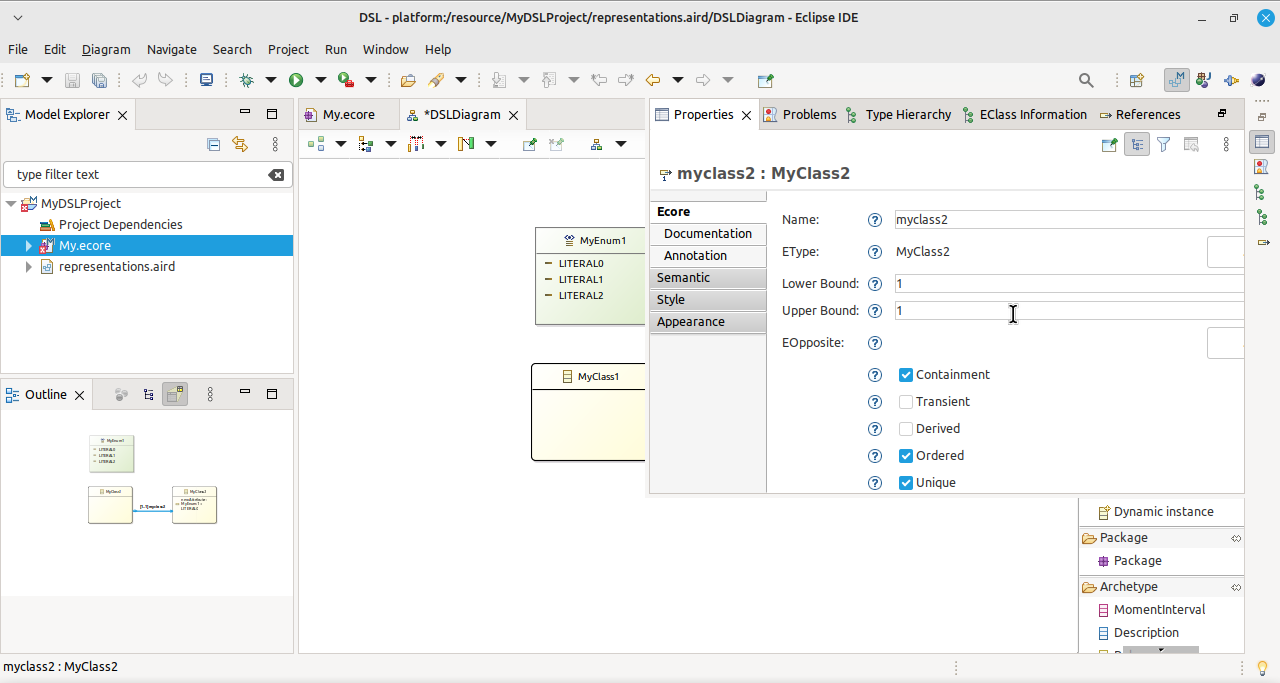
\includegraphics[width=\ScreenshotWidth\textwidth]{./Screenshots/SS_20.png}
\caption{The properties menu is a small button on the right side.}
\label{fig:SSOpenedPropertiesMenu}
\end{figure}




\end{document}
%%%%% %%%%% %%%%% %%%%% %%%%% %%%%% %%%%% %%%%%              %%%%% %%%%% %%%%% %%%%% %%%%% %%%%% %%%%% %%%%%
%%%%% %%%%% %%%%% %%%%% %%%%% %%%%% %%%%% %%%%% END document %%%%% %%%%% %%%%% %%%%% %%%%% %%%%% %%%%% %%%%%
%%%%% %%%%% %%%%% %%%%% %%%%% %%%%% %%%%% %%%%%              %%%%% %%%%% %%%%% %%%%% %%%%% %%%%% %%%%% %%%%%
